\date{}
\title{CSO2: Caching}
\date{}



\begin{document}

\usepgflibrary{shapes.gates.logic.mux}
\input{../common/listingsLib}
\newcommand{\z}[2]{\only<#1->{\myemph<#1>{#2}}}
\newcommand{\zz}[3]{\only<#1-#2>{\myemph<#1>{#3}}}
\newcommand{\zzx}[3]{\only<#1-#2>{#3}}
\newlength{\oneZero}
\settowidth{\oneZero}{\small\tt 0}
\newlength{\twoZeroes}
\settowidth{\twoZeroes}{\small\tt 00}




\begin{frame}{Agenda}
    \begin{itemize}
        \item Logistics
            \begin{itemize}
            \item Labs this week (\texttt{signals} lab)
            \item \textbf{timing} homework due next Friday (uses signals)
            \end{itemize}
        \item Last time: where do processes come from?
        \item This time: how do parent-child processes interact?
            \begin{itemize}
                \item waiting on processes
                \item file descriptors
            \end{itemize}
    \end{itemize}
\end{frame}


% \begin{frame}{last time?}
% \begin{center}
%     \includegraphics[width=0.4\pagewidth]{fork.jpg}
% \end{center}
% \end{frame}
% \begin{frame}{last time?}
% \begin{center}
%     \includegraphics[width=0.7\pagewidth]{forkroad.jpg}
% \end{center}
% \end{frame}


% 
\usetikzlibrary{matrix,patterns,arrows.meta,decorations.pathreplacing}
\begin{frame}{\texttt{fork}}
\begin{itemize}
\item \texttt{pid\_t fork()} --- copy the current process
\item returns twice:
    \begin{itemize}
    \item in \textit{parent} (original process): pid of new \textit{child} process
    \item in \textit{child} (new process): \texttt{0}
    \end{itemize}
\item \myemph{everything (but pid) duplicated} in parent, child:
    \begin{itemize}
    \item memory
    \item file descriptors (later)
    \item registers
    \end{itemize}
\end{itemize}
\end{frame}





\subsection{exercises: multi-level lookup}
% % FIXME: \subsubsection{part 0}
% % FIXME: \input{../vm/multiSplitExPt0}
% \subsubsection{part 2}
% \usetikzlibrary{matrix,positioning}

\begin{frame}{2-level splitting}
    \begin{itemize}
    \item 9-bit virtual address 
    \item 6-bit physical address
    \item<2-> \myemph<2>{8-byte pages $\rightarrow$ 3-bit page offset (bottom)}
    \item<2-> 9-bit VA: 6 bit VPN + 3 bit PO
    \item<2-> 6-bit PA: 3 bit PPN + 3 bit PO
    \item<3-> \myemph<3>{1 page page tables w/ 1 byte entry $\rightarrow$ 8 entry PTs}
    \item<4-> \myemph<4>{8 entry page tables $\rightarrow$ 3-bit VPN parts}
    \item<4-> 9-bit VA: 3 bit VPN part 1; 3 bit VPN part 2
    \end{itemize}
\begin{tikzpicture}[overlay,remember picture]
    \coordinate (begin) at ([xshift=-1cm,yshift=-2cm]current page.north east);
    \tikzset{
        page offset/.style={alt=<2>{draw=red,fill=red!10}},
    }
    \begin{scope}[shift={(begin)},x=1.25cm] 
        \draw (-6, 0) rectangle (0, 0.5);
        \node[anchor=south] at (-3, 0.4) {virtual addr};
        \begin{visibleenv}<2-3>
        \draw (-6, 0) rectangle (-2, 0.5) node[midway] {VPN};
        \end{visibleenv}
        \begin{visibleenv}<4->
        \draw (-6, 0) rectangle (-2, 0.5);
            \draw[alt=<4>{red},dotted] (-6, 0) rectangle (-4, 0.5) node[midway,font=\fontsize{11}{12}\selectfont] {VPN pt 1};
            \draw[alt=<4>{red},dotted] (-4, 0) rectangle (-2, 0.5) node[midway,font=\fontsize{11}{12}\selectfont] {VPN pt 2};
        \end{visibleenv}
        \begin{visibleenv}<2->
        \draw[page offset] (-2, 0) rectangle (0, 0.5) node[midway] {page offset};
        \end{visibleenv}
        \begin{scope}[every node/.style={font=\fontsize{10}{11}\selectfont\tt,inner sep=0mm}]
            \node[anchor=north] at (0, 0) {0};
            \node[anchor=north] at (-2, 0) {3};
            \node[anchor=north] at (-4, 0) {6};
            \node[anchor=north] at (-6, 0) {9};
        \end{scope}
        \begin{scope}[yshift=-1.5cm]
            \draw (-4, 0) rectangle (0, 0.5);
            \node[anchor=south] at (-2, 0.4) {physical addr};
            \begin{visibleenv}<2->
            \draw (-4, 0) rectangle (-2, 0.5) node[midway] {PPN};
            \draw[page offset] (-2, 0) rectangle (0, 0.5) node[midway] {page offset};
            \end{visibleenv}
            \begin{scope}[every node/.style={font=\fontsize{10}{11}\selectfont\tt,inner sep=0mm}]
                \node[anchor=north] at (0, 0) {0};
                \node[anchor=north] at (-2, 0) {3};
                \node[anchor=north] at (-4, 0) {6};
            \end{scope}
        \end{scope}
        \begin{visibleenv}<3->
        \begin{scope}[yshift=-4cm]
            \matrix[tight matrix,
                nodes={text width=1cm,font=\small},
                column 1/.style={nodes={text width=0.6cm,draw=none}},
                row 1/.style={nodes={draw=none}},
                label={north:page table \small (either level)},
            ] at (-1, 0){
                ~ \& valid? \& PPN \\
                0 \& ~ \& ~ \\
                1 \& ~ \& ~ \\
                2 \& ~ \& ~ \\
                \ldots \& |[draw=none]|\ldots \& |[draw=none]|\ldots \\
                \myemph<4>{7} \& ~ \& ~ \\
            };
        \end{scope}
        \end{visibleenv}
    \end{scope}
\end{tikzpicture}
\end{frame}

\begin{frame}{2-level example}
\begin{itemize}
\item {}\myemph<1>{9-bit} virtual addresses, 6-bit physical; 8 byte pages, 1 byte PTE
\item page tables 1 page; PTE: 3 bit PPN (MSB), 1 valid bit, 4 unused
\item page table base register {\tt 0x20}; translate virtual address {\tt 0x129}
\end{itemize}
\begin{tikzpicture}
\matrix[tight matrix,anchor=north west,
    nodes={text width=2cm,minimum height=0.5cm,font=\small},
    column 1/.style={nodes={draw=none,font=\small\tt,align=right}},
    column 2/.style={nodes={draw,thick,font=\small\tt,text width=2.6cm,align=left}},
    row 1/.style={nodes={draw=none,font=\small\normalfont}},
    ] (memA)  {
    physical addresses \& bytes \\
    0x00-3 \& 00 11 22 33 \\
    0x04-7 \& 44 55 66 77 \\
    0x08-B \& 88 99 AA BB \\
    0x0C-F \& CC DD EE FF \\
    0x10-3 \& 1A 2A 3A 4A \\
    0x14-7 \& 1B 2B 3B 4B \\
    0x18-B \& 1C 2C 3C 4C \\
    0x1C-F \& 1C 2C 3C 4C \\
};
\matrix[tight matrix,anchor=north west,
    nodes={text width=2cm,minimum height=0.5cm,font=\small},
    column 1/.style={nodes={draw=none,font=\small\tt,align=right}},
    column 2/.style={nodes={draw,thick,font=\small\tt,text width=2.6cm,align=left}},
    row 1/.style={nodes={draw=none,font=\normalfont\small}},
    ] (memB) at ([xshift=0cm]memA.north east) {
    physical addresses \& bytes \\
    0x20-3 \& 00 91 72 13 \\
    0x24-7 \& \maybeEmph<2>{F4} A5 36 07 \\
    0x28-B \& 89 9A AB BC \\
    0x2C-F \& CD DE EF F0 \\
    0x30-3 \& BA \maybeEmph<5>{0A} BA 0A \\
    0x34-7 \& DB 0B DB 0B \\
    0x38-B \& EC 0C EC 0C \\
    0x3C-F \& AC \maybeEmph<3>{DC} DC 0C \\
};
\iftoggle{heldback}{}{
\begin{visibleenv}<2->
\node[right=0cm of memB,align=left,font=\small] {
    {\tt 0x129} = {\tt \myemph<2>{\color<6>{blue}1 00}\myemph<3>{\color<6>{violet}10 1}\myemph<5>{\color<6>{orange}001}} \\
    \texttt{0x20} + {\color<6>{blue}\tt 0x4}~\times 1 = {\tt 0x24} \\
    \textit{PTE 1 value:} \\
    {\tt 0xF4} = {\tt 1111 0100} \\
    PPN {\tt {\color<6>{green} 111}}, valid {\tt 1} \\
    \only<3->{\textit{PTE 2 addr:}} \\
    \only<3->{\texttt{{\color<6>{green} 111} 000} +  \texttt{\myemph<3>{\color<6>{violet} 101}} $\times$ 1 = {\tt 0x3D}}\\
    \only<3->{\textit{PTE 2 value:} {\tt 0xDC}} \\
    \only<4->{PPN {\tt \myemph<4>{\color<6>{red}110}}; valid {\tt 1}} \\
    \only<4->{M[\texttt{\myemph<4>{\color<6>{red}110} \myemph<5>{\color<6>{orange}001}} (\texttt{0x31})] = \texttt{0x0A}}
};
\end{visibleenv}
}
\end{tikzpicture}
\end{frame}

% \subsubsection{part 3}
% \input{../vm/multiSplitExPt3}
% \input{../vm/multiSplitExPt3b}
% \subsubsection{part 4}
% \input{../vm/multiSplitExPt4}
\subsubsection{part 5}
\input{../vm/multiSplitExPt5}



\begin{frame}
    \titlepage
\end{frame}



\begin{frame}{Building our toolkit}
    \begin{itemize}
        \item Access to system resources (e.g., files)
            \begin{itemize}
            \item system calls
            \item user IDs and permissions
            \end{itemize}

        \item Handling events (e.g., timer firing) and sharing CPU
            \begin{itemize}
                \item exceptions
                \item context switches
            \end{itemize}

        \item Creating new processes and shell operations
            \begin{itemize}
                \item fork(), exec()
                \item file descriptors
            \end{itemize}

        \item Strict process isolation
            \begin{itemize}
                \item virtual memory
            \end{itemize}

        \item next: Increasing memory performance
            \begin{itemize}
                \item caching
            \end{itemize}

    \end{itemize}
\end{frame}




\section{caching intro}

\subsection{memory hierarchy intro}
\input{../caching/memHierarchyIntro}

\subsection{locality}
\input{../caching/localityBasics}

\subsection{typical cache hierarchy}
\usetikzlibrary{arrows.meta,calc,patterns}

\begin{frame}{split caches; multiple cores}
\begin{tikzpicture}
    \tikzset{
        >=Latex,
        connect/.style={<->,ultra thick},
        cache/.style={draw,very thick,align=center},
    }
\node[cache] (icache1) {instr. \\ cache \\ (core 1)};
\node[cache,anchor=west] (dcache1) at ([xshift=2cm]icache1.east) {data \\ cache \\ (core 1)};
\node[cache] (icache2) {instr. \\ cache \\ (core 1)};
\node[cache,anchor=west] (icache2) at ([xshift=3cm]dcache1.east) {instr. \\ cache \\ (core 2)};
\node[cache,anchor=west] (dcache2) at ([xshift=2cm]icache2.east) {data \\ cache \\ (core 2)};
\node[cache, minimum width=4cm,anchor=north] (l21) at ([yshift=-1cm]$(icache1.south)!0.5!(dcache1.south)$) {unified \\ L2 cache \\ (core 1)};
\node[cache, minimum width=4cm,anchor=north] (l22) at ([yshift=-1cm]$(icache2.south)!0.5!(dcache2.south)$) {unified \\ L2 cache \\ (core 2)};
    \node[cache, minimum width=8cm,anchor=north] (l3) at ([yshift=-1cm]$(l21.south)!0.5!(l22.south)$) {L3 cache \\ (shared between cores)};
\foreach \fromC/\toC in {icache1/l21,dcache1/l21,icache2/l22,dcache2/l22,l21/l3,l22/l3} {
\draw[connect] (\fromC.south) -- ++(-0cm,-.5cm) -| (\toC.north);
}
\end{tikzpicture}
\end{frame}

\begin{frame}{hierarchy and instruction/data caches}
    \begin{itemize}
    \item typically separate data and instruction caches for L1
    \vspace{.5cm}
    \item (almost) never going to read instructions as data or vice-versa
    \item avoids instructions evicting data and vice-versa
    \item can optimize instruction cache for different access pattern
    \item easier to build fast caches: that handles less accesses at a time
    \end{itemize}
\end{frame}



\subsection{one-block cache}
\input{../caching/oneBlockCache}

\subsection{direct mapped caches}
\input{../caching/directMappedIntro}

\begin{frame}{terminology}
    \begin{itemize}
    \item row = set
        \begin{itemize}
        \item preview: change how much is in a row
        \end{itemize}
    \end{itemize}
\end{frame}

\subsection{tag/index/offset for direct mapped caches}
\input{../caching/tioDMIntro}

\subsubsection{aside: cache size}
\begin{frame}{cache size}
    \begin{itemize}
    \item cache size = amount of \textit{data} in cache
    \item not included metadata (tags, valid bits, etc.)
    \end{itemize}
\end{frame}

\subsection{prelim. formulas}
\begin{frame}{Tag-Index-Offset formulas (direct-mapped only)}
\def\arraystretch{1.5}
\begin{tabular}{ll}
$m$ & memory addreses bits \\
$S=2^s$ & number of sets \\
$s$  & (set) index bits \\
$B=2^b$ & block size \\
$b$ & (block) offset bits \\
$t = m - (s+b)$ & tag bits \\
$C = B \times S$ & cache size (if direct-mapped) \\
\end{tabular}
\end{frame}


\subsection{tio for DM: exercise}
\input{../caching/tioDmExercise}

\subsection{simulating a direct mapped cache}
\input{../caching/dmExampleAccess}

\subsection{exercise: direct-mapped cache access}
\input{../caching/dmAccessExercise}

\subsection{mapping misses to sets (DM)}
\input{../caching/setMappingDiagDM}

\subsection{cache misses on real code}
\begin{frame}{actual misses: BST lookups}
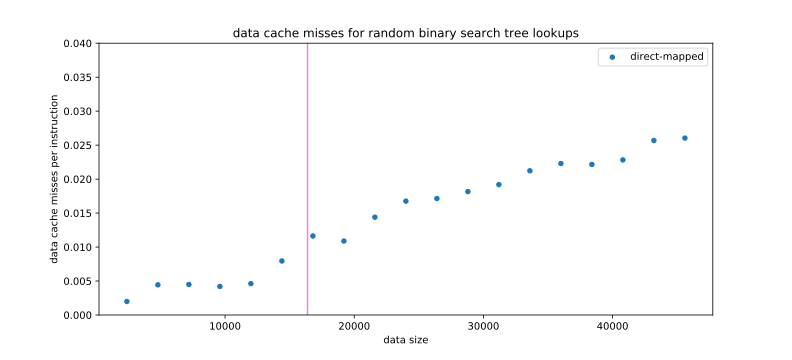
\includegraphics[width=\textwidth]{../caching/bst-one}
\end{frame}

\begin{frame}{actual misses: matrix multiplies}
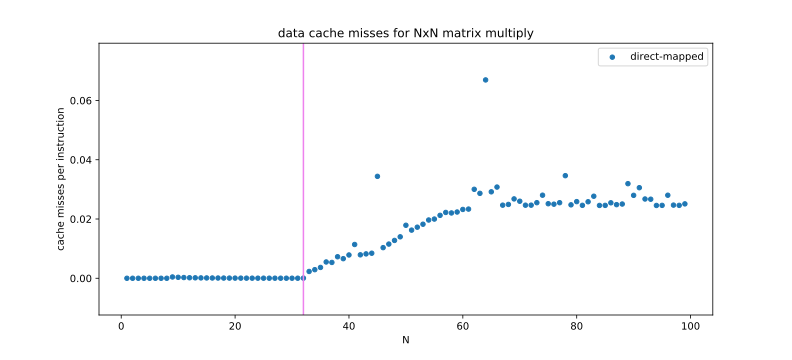
\includegraphics[width=\textwidth]{../caching/mm-one}
\end{frame}


\section{adding associativity}
\input{../caching/addAssoc}

\subsection{diagram}
\usetikzlibrary{decorations,decorations.pathreplacing,circuits.logic.US,matrix,positioning,fit}
\usetikzlibrary{circuits.logic.mux}

\begin{frame}{cache operation (associative)}
\begin{tikzpicture}[circuit logic US]
\tikzset{
    myline/.style={-latex,thick},
    myline thin/.style={-latex,thin},
    myline bus/.style={-latex,ultra thick},
    myline no arrow/.style={thick},
    offsetColor/.style={color=yellow!30!black},
    tagColor/.style={color=green!60!black},
    tagStoreFill/.style={fill=green!20},
    tagColorFill/.style={tagColor,fill=green!60!black},
    dataColor/.style={color=blue!60!black},
    dataColorFill/.style={tagColor,fill=blue!60!black},
    dataStoreFill/.style={fill=blue!20},
    triangle down/.style = {draw,regular polygon, regular polygon sides=3, shape border rotate=180},
}
\matrix[tight matrix,
        nodes={draw,
               font=\small\tt,
               text depth=0.2ex,
               text height=1.4ex,
        },
        row 1/.style={nodes={font=\small\bfseries}},
        column 1/.style={nodes={text width=1cm,align=center}},
        column 2/.style={nodes={text width=1cm,tagColor,tagStoreFill}},
        column 3/.style={nodes={text width=1.3cm,dataColor,dataStoreFill}},
        column 4/.style={nodes={text width=.1cm,draw=none}},
        column 5/.style={nodes={text width=1cm,align=center}},
        column 6/.style={nodes={text width=1cm,tagColor,tagStoreFill}},
        column 7/.style={nodes={text width=1.3cm,dataColor,dataStoreFill}},
        ] (cache) {
    valid \& tag \&  data \& ~ \& valid \& tag \& data\\
    1  \& 10 \& 00 11 \& ~ \& 1 \& 00 \& AA BB \\
    ~ \& ~ \& ~ \&   ~ \&  ~ \& ~ \& ~\\
    ~ \& ~ \& ~ \&   ~ \&  ~ \& ~ \& ~\\
    ~ \& ~ \& ~ \&   ~ \&  ~ \& ~ \& ~\\
    1 \&  11 \& B4 B5 \& ~ \& 1 \& 01 \& 33 44 \\
    ~ \& ~ \& ~ \&   ~ \&  ~ \& ~ \& ~\\
    ~ \& ~ \& ~ \&   ~ \&  ~ \& ~ \& ~\\
    ~ \& ~ \& ~ \&   ~ \&  ~ \& ~ \& ~\\
};
\begin{scope}[every node/.style={draw,rectangle,dashed,inner xsep=0pt,outer sep=0pt,font=\tt}]
\node (idx) at ([yshift=1cm,xshift=-.3cm]cache.north west){100};
\node[left=0cm of idx,tagColor] (tag) {11};
\node[right=0cm of idx,offsetColor] (offset) {1};
\end{scope}
\draw[thick,dashed,-latex] (idx) |- ([xshift=-.2cm]cache-6-1.north west) node[near start,font=\small,fill=white,inner sep=2pt,xshift=-.3cm] {index};
\draw[very thick,decorate,decoration={brace,mirror},overlay] ([xshift=-.1cm]cache-2-1.north west) -- ([xshift=-.1cm]cache-9-1.south west);

\node[fit=(cache-6-1) (cache-6-7),inner sep=1pt,red,draw,line width=3pt] {};

\draw[thick,dashed,-latex,tagColor] (tag) |- ([yshift=-.5cm]cache-9-2.south) coordinate (tag cmp 1);
\draw[thick,dashed,-latex,tagColor] (cache-9-2.south) -- (tag cmp 1);
\draw[thick,dashed,-latex,tagColor] (tag) |- ([yshift=-1cm]cache-9-6.south) coordinate (tag cmp 2)
    node[pos=0.25,fill=white] {tag};
\draw[thick,dashed,-latex,tagColor] (cache-9-6.south) -- (tag cmp 2);

\draw[thick,dashed,-latex,offsetColor] (offset.south) -- ++(0cm, -.1cm) -| ([yshift=.2cm]cache-1-3.north);
\draw[thick,dashed,-latex,offsetColor] (offset.south) -- ++(0cm, -.1cm) -| ([yshift=.2cm]cache-1-7.north);

\draw[very thick,decorate,decoration={brace,mirror},overlay] ([yshift=.1cm]cache-1-3.north east) -- ([yshift=.1cm]cache-1-3.north west);
\draw[very thick,decorate,decoration={brace,mirror},overlay] ([yshift=.1cm]cache-1-7.north east) -- ([yshift=.1cm]cache-1-7.north west);

\end{tikzpicture}
% FIXME: place diagram here
\end{frame}


\subsection{options for replacement}
\input{../caching/replacement}

\subsection{associativity terms}
\input{../caching/assocTerms}

\subsection{tag/index/offset for set-assoc. caches}
\begin{frame}{Tag-Index-Offset formulas}
\def\arraystretch{1.5}
\begin{tabular}{ll}
$m$ & memory addreses bits \\
$E$ & number of blocks per set (``ways'') \\
$S=2^s$ & number of sets \\
$s$  & (set) index bits \\
$B=2^b$ & block size \\
$b$ & (block) offset bits \\
$t = m - (s+b)$ & tag bits \\
$C = B \times S \times E$ & cache size (excluding metadata) \\
\end{tabular}
\end{frame}




\end{document}
